%----------------------------------------------------------------------------------------
%	PACKAGES AND OTHER DOCUMENT CONFIGURATIONS
%----------------------------------------------------------------------------------------

\documentclass[paper=a4, fontsize=11pt]{scrartcl} % A4 paper and 11pt font size
\usepackage{listings}
\usepackage{color}
	
\definecolor{codegreen}{rgb}{0,0.6,0}
\definecolor{codegray}{rgb}{0.5,0.5,0.5}
\definecolor{codepurple}{rgb}{0.58,0,0.82}
\definecolor{backcolour}{rgb}{0.95,0.95,0.92}
	
\lstdefinestyle{mystyle}{
	backgroundcolor=\color{backcolour},   
	commentstyle=\color{codegreen},
	keywordstyle=\color{magenta},
	numberstyle=\tiny\color{codegray},
	stringstyle=\color{codepurple},
	basicstyle=\footnotesize,
	breakatwhitespace=false,         
	breaklines=true,                 
	captionpos=b,                    
	keepspaces=true,                 
	numbers=left,                    
	numbersep=5pt,                  
	showspaces=false,                
	showstringspaces=false,
	showtabs=false,                  
	tabsize=2
}
	
\lstset{style=mystyle}
\usepackage[T1]{fontenc} % Use 8-bit encoding that has 256 glyphs
\usepackage{fourier} % Use the Adobe Utopia font for the document - comment this line to return to the LaTeX default
\usepackage[english]{babel} % English language/hyphenation
\usepackage{amsmath,amsfonts,amsthm} % Math packages
\usepackage{graphicx}
\usepackage{hyperref}
\usepackage{sectsty} % Allows customizing section commands
\allsectionsfont{\normalfont \scshape} % Make all sections centered \centering, the default font and small caps
\usepackage{csquotes}
\usepackage{fancyhdr} % Custom headers and footers
\usepackage{subcaption}
\pagestyle{fancyplain} % Makes all pages in the document conform to the custom headers and footers
\fancyhead{} % No page header - if you want one, create it in the same way as the footers below
\fancyfoot[L]{} % Empty left footer
\fancyfoot[C]{} % Empty center footer
\fancyfoot[R]{\thepage} % Page numbering for right footer
\renewcommand{\headrulewidth}{0pt} % Remove header underlines
\renewcommand{\footrulewidth}{0pt} % Remove footer underlines
\setlength{\headheight}{13.6pt} % Customize the height of the header

\numberwithin{equation}{section} % Number equations within sections (i.e. 1.1, 1.2, 2.1, 2.2 instead of 1, 2, 3, 4)
\numberwithin{figure}{section} % Number figures within sections (i.e. 1.1, 1.2, 2.1, 2.2 instead of 1, 2, 3, 4)
\numberwithin{table}{section} % Number tables within sections (i.e. 1.1, 1.2, 2.1, 2.2 instead of 1, 2, 3, 4)

\setlength\parindent{0pt} % Removes all indentation from paragraphs - comment this line for an assignment with lots of text

%----------------------------------------------------------------------------------------
%	TITLE SECTION
%----------------------------------------------------------------------------------------

\newcommand{\horrule}[1]{\rule{\linewidth}{#1}} % Create horizontal rule command with 1 argument of height

\title{	
\normalfont \normalsize 
\textsc{Udacity, Robotics Nano Degree} \\ [25pt] % Your university, school and/or department name(s)
\horrule{0.5pt} \\[0.4cm] % Thin top horizontal rule
\huge Follow Me \\ % The assignment title
\horrule{2pt} \\[0.5cm] % Thick bottom horizontal rule
}

\author{Myoungki Jung} % Your name

\date{\normalsize\today} % Today's date or a custom date

\begin{document}

\maketitle % Print the title

\section{Neural Network Architecture}

\subsection{Fully Convolutional Neural networks}

The use of fully convolutional network allowed to conduct scene segmentation for images. 
Previously, convolutional neural networks were used in classification of images such as MNIST, and Imagenet. However, these normal convolutional network only supports in classification.
\href{https://www.facebook.com/yann.lecun/posts/10152820758292143}{Yann LeCun} stated that:

\begin{displayquote}
	In Convolutional Nets, there is no such thing as “fully-connected layers”. There are only convolution layers with 1x1 convolution kernels and a full connection table.
\end{displayquote}

It is essential an autoencoder replaced the middle fully-connected layers with 1x1 convoluion layer.

\subsubsection{encoder}
\begin{figure}[htp]
	\centering
	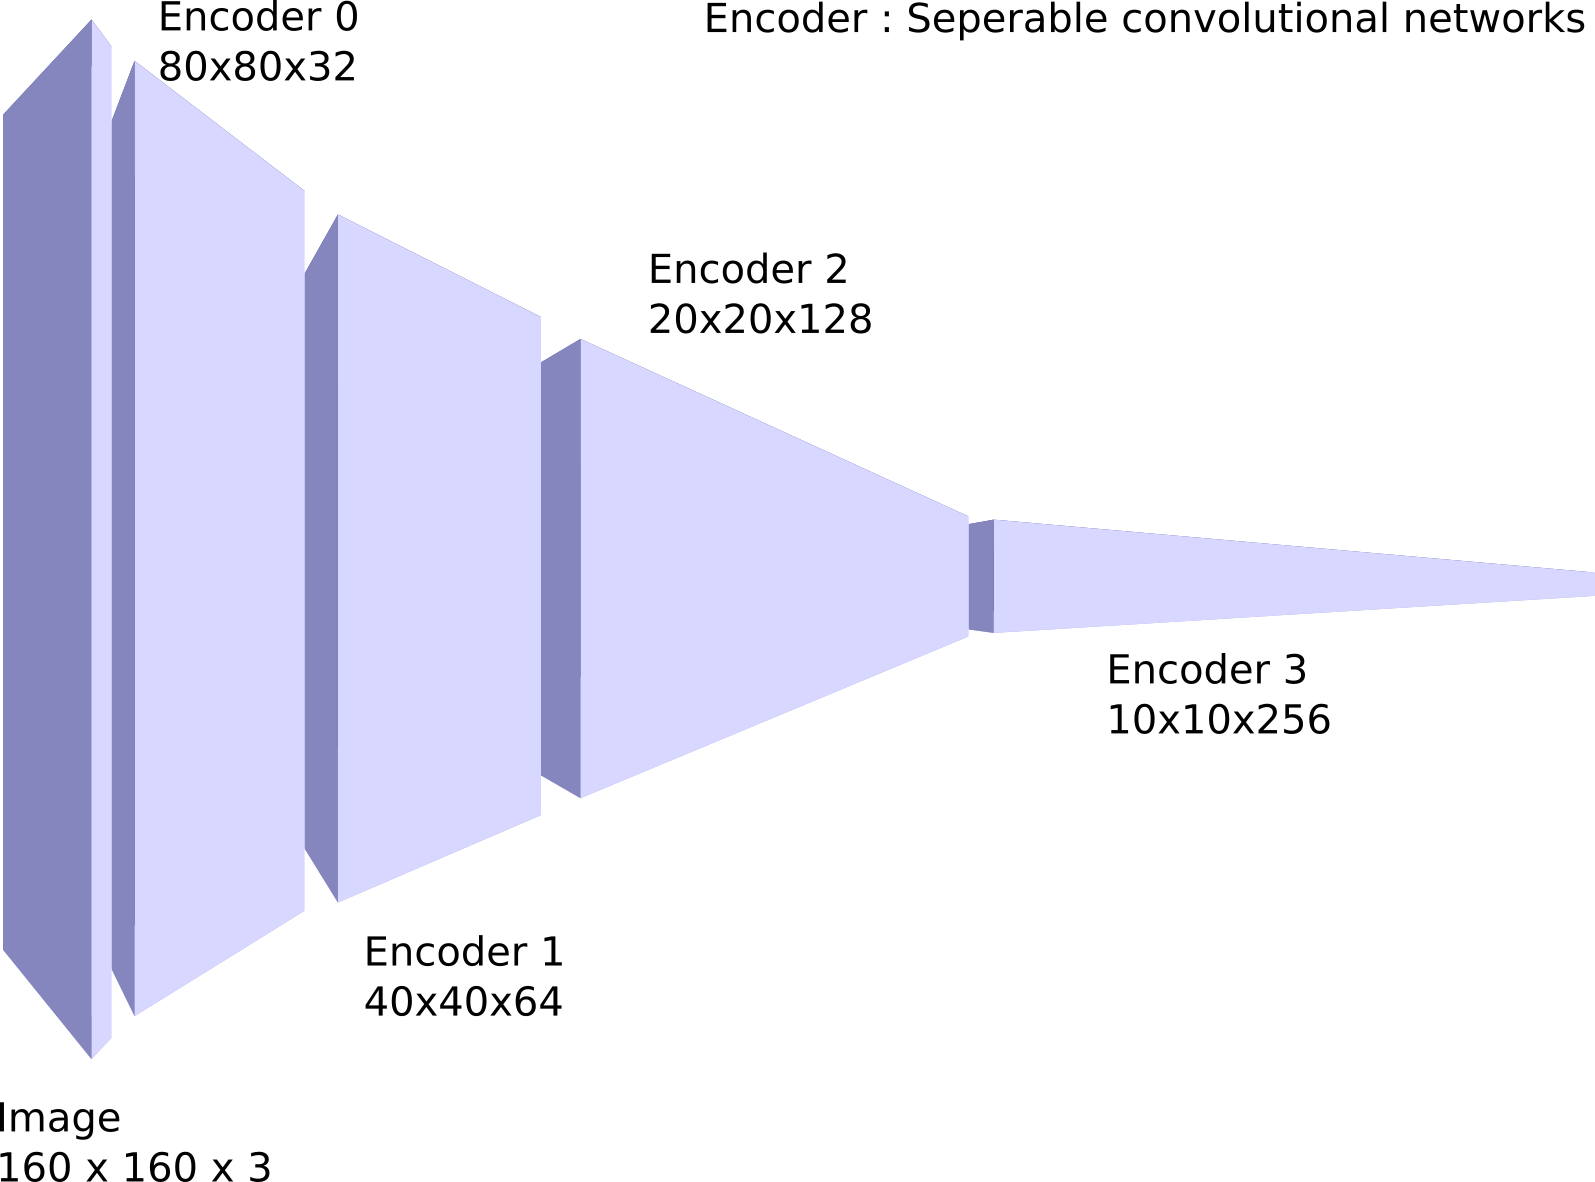
\includegraphics[scale=0.2]{./imgs/encoder.png}
	\caption{Fully connected convolutional network used in the project}
	\label{fig:encoder}
\end{figure}
\begin{lstlisting}[language=Python, caption= Endcoder block code]
	def encoder_block(input_layer, filters, strides):

		output_layer = separable_conv2d_batchnorm(input_layer, filters, strides)

    return output_layer
\end{lstlisting}
Encoder consists of four layers of neural network modules and each module consists of a separable convolution layer. Later a conv2d\_batchnorm with the same filter size was applied in the FCN model. 
\paragraph{encoding} Once this parts are trained this encodes the image into the input to the 1x1 convolution layer, which contains the activated weights of the image. During the encoding process, some information may be lost due to the coarse strides of convolution or pooling layer and the type of pooling ( average, max).

\paragraph{seperable convolution} The separable convolutional network is the key part which reduces the number of parameters needed to increase efficiency for the encoder network. The seperable convolutional network includes a convolutional network, and an activation function.
The function used in the encoder module is class SeparableConv2DKeras and it performs depthwise spatial convolution and a pointwise convolution and controls output depth. In short, it is a way to factorize a convolution kernel into two smaller kernels.

\paragraph{why not fully connected layer?} Fully connected layer is usually used to evaluate the neural network weights before sending it to activation layer, for classification classification. The output of this layer loses the spatial information contained in the convolutional networks and this cannot be used in our application as the network needs to contain the spatial network information to reproduce the scene segmentation as output

\paragraph{1x1 convolution} Google used this in their \href{https://arxiv.org/abs/1409.4842}{Inception paper} to reduce the computational load but still make the network deeper.

\begin{displayquote}
	in our setting, 1x1 convolutions have dual purpose: most critically, they are used mainly as dimension reduction modules to remove computational bottlenecks, that would otherwise limit the size of our networks. This allows for not just increasing the depth, but also the width of our networks without significant performance penalty.
\end{displayquote}

\href{https://iamaaditya.github.io/2016/03/one-by-one-convolution/}{Aaditya Prakash} also discussed 1x1 convolution in his github blog that this convolution is a strictly linear coordinate-dependent transformation in the filter space which leads to dimensionality reduction and increase in depth of network. It is also less likely experiencing over-fitting because of its small 1x1 kernel size. 

\subsubsection{decoder}
\begin{figure}[htp]
	\centering
	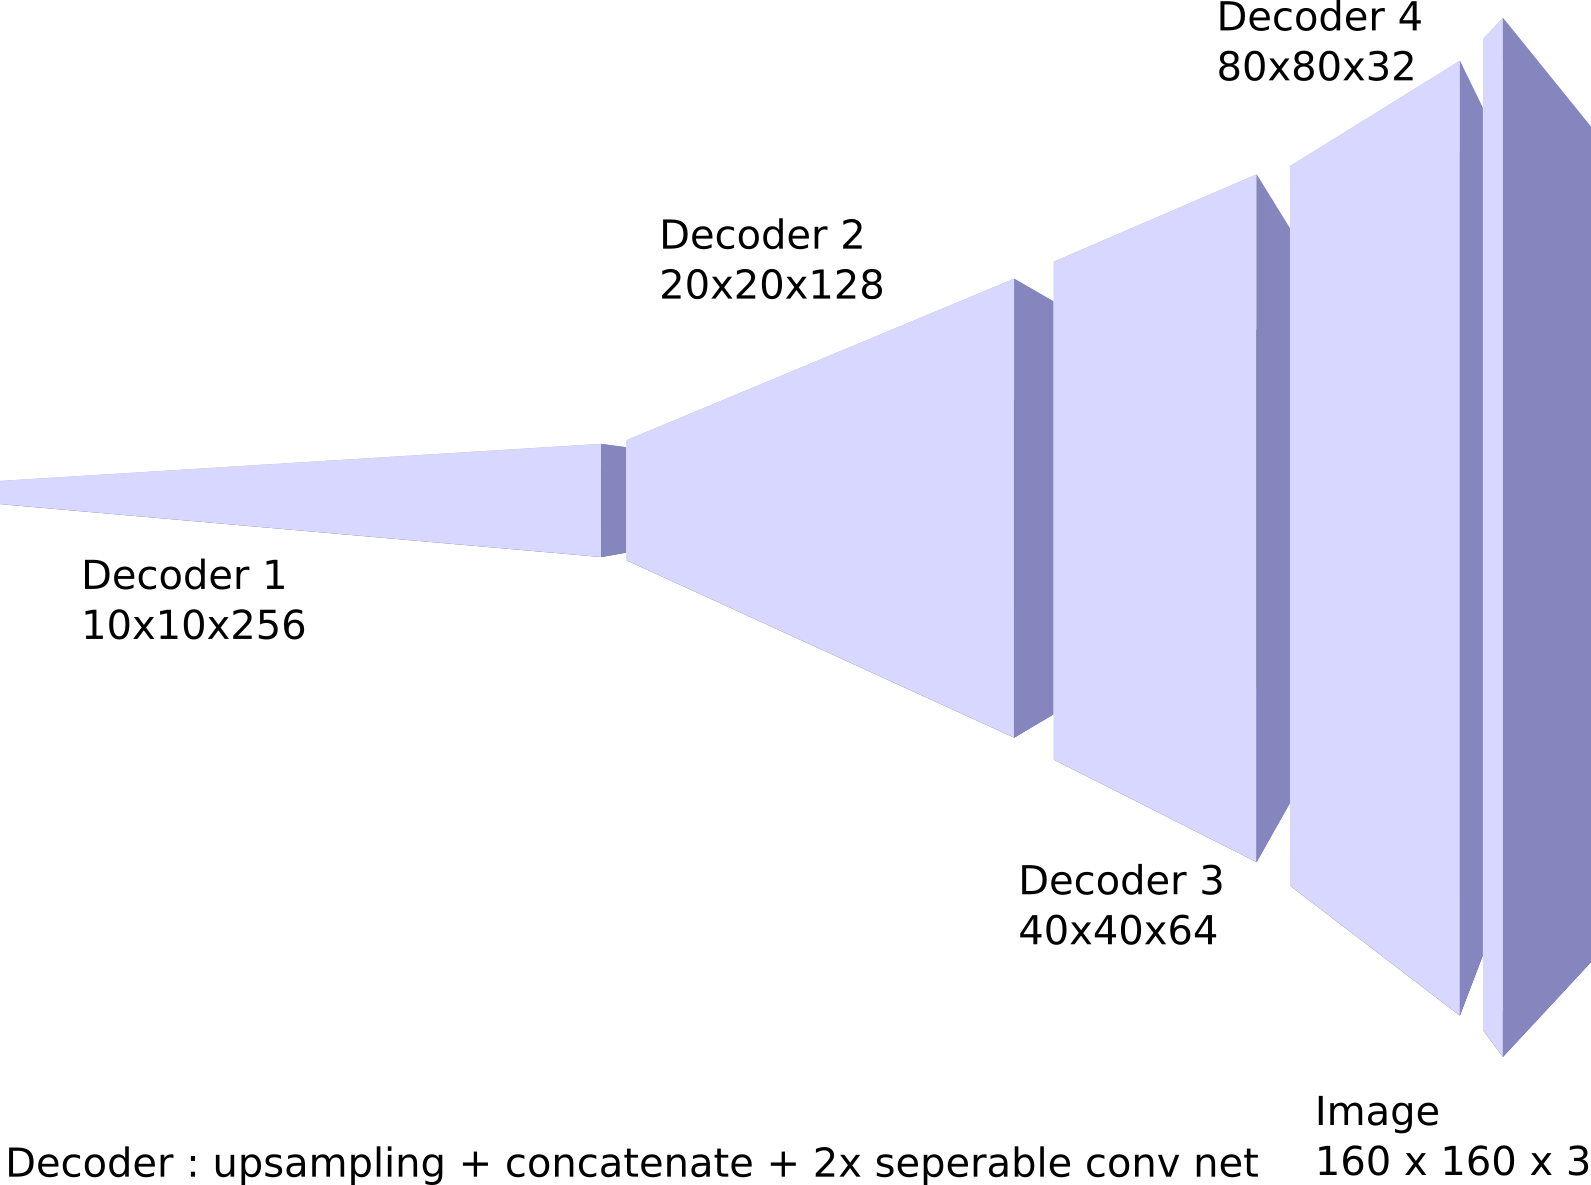
\includegraphics[scale=0.2]{./imgs/decoder.png}
	\caption{Fully connected convolutional network used in the project}
	\label{fig:decoder}
\end{figure}

Decoder is more complicated than the encoder. This block consists of an upsampling layer, concatenate filter, and two separable\_conv2d\_batchnorm layers.
\begin{lstlisting}[language=Python, caption=Decoder block code]
	def decoder_block(small_ip_layer, large_ip_layer, filters):
    
		upsampled_output_layer = bilinear_upsample(small_ip_layer)
		
		output_layer = layers.concatenate([upsampled_output_layer,large_ip_layer])
		
		output_layer = separable_conv2d_batchnorm(output_layer, filters)
		output_layer = separable_conv2d_batchnorm(output_layer, filters)
    
    return output_layer
\end{lstlisting}

\paragraph{upsampling} The upsampling layer uses BilinearUpSampling2D, which repeats the rows and columns of the data, in this case 2x2. This upsampling increases the size of the matrix back to original output size by applying the same number of separable\_conv2d\_batchnorm in the encoder block.
\paragraph{concatenate} tensorflow's concatenate connects the output layer of upsampling function and the equivalent sized encoder block.
\paragraph{separable convolution} is the same as ones in the encoder blocks.
\paragraph{decoding} Decoding of an image from the information inside 1x1 convolution layer is done by multiple upsampling.

\subsubsection{Fully connected convolutional network}
FCN consists of multiple blocks of encoder and decoder, and 1x1 convolution layer. Differently from the normal convolutional neural networks, a seperable network links a pair of enconders and decoders and creates sharper image output as shown in the lesson.

\paragraph{Chosen Architecture}
The Architecture of the Neural network is Fully connected convolutional network (FCN). This network can decode the weights in the newural network back to an image, which shows the true and false in pixels. This decoding capability enables the scene segmentation, identification of target object in this project.

\begin{figure}[htp]
	\centering
	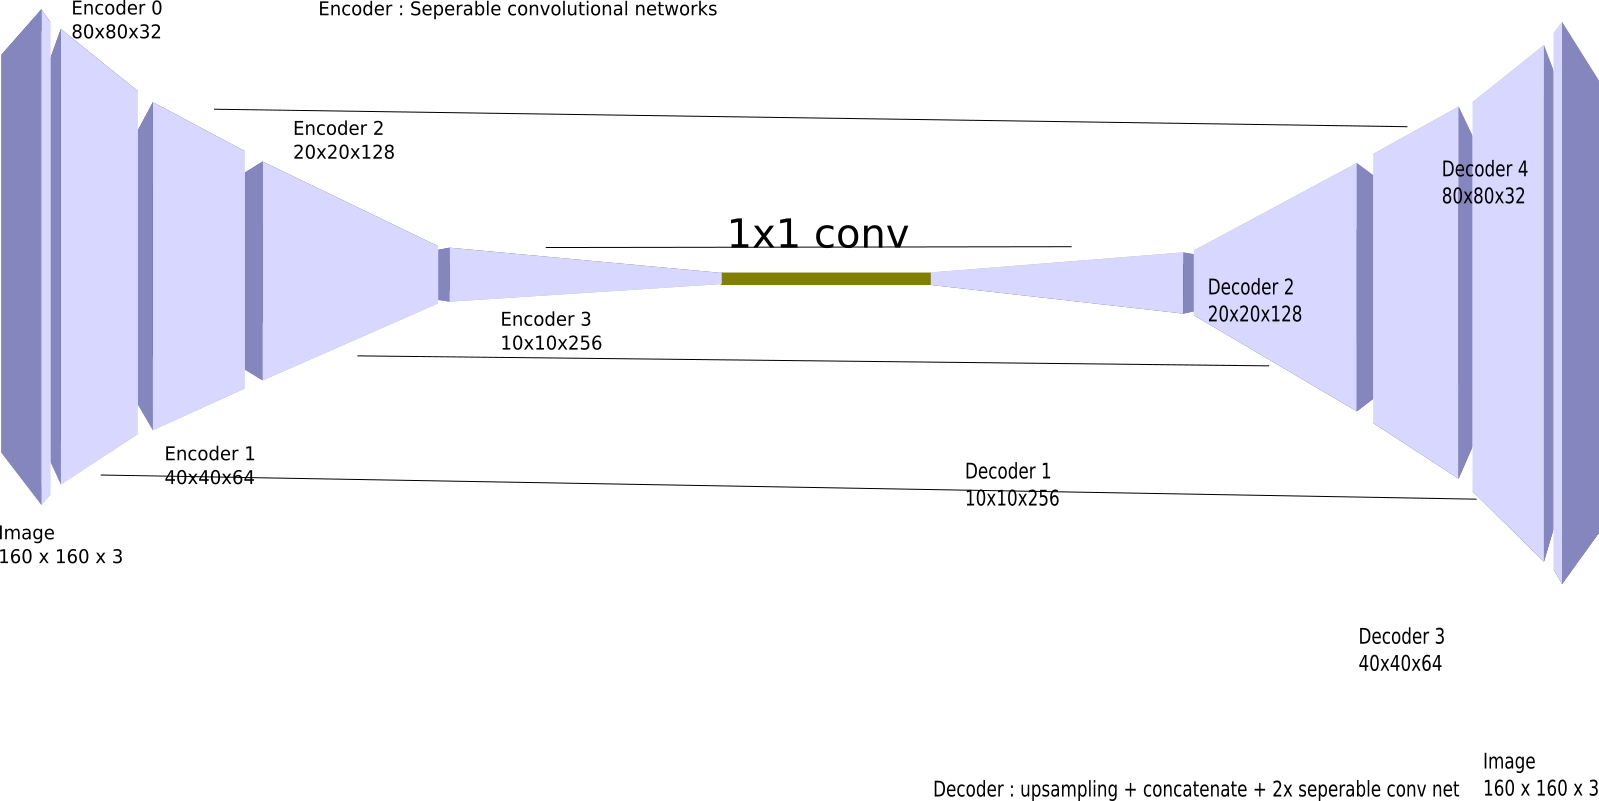
\includegraphics[scale=0.35]{./imgs/FCN.png}
	\caption{Fully connected convolutional network used in the project}
	\label{fig:FCN}
\end{figure}
The gold colour component in Figure~\ref{fig:FCN}, 1x1 convolution layer was used to make it as an adaptor filter between encoder and decoder module beacuse this filter stil conveys weights with the spatial data in the previous filters, unlike the classifer losing all the data and flattened, and only reduce dimension of the matrix, which removes computational bottlenecks. 1x1 convolution was used after 'relu' layer of 'SeparableConv2DKeras' to reduce the dimensions and to prepare for connections to following seperable convolution layers.

\begin{lstlisting}[language=Python, caption=Fully convolutional network code]
	def fcn_model(inputs, num_classes):

		filter= 32
		
		encoded_0 = encoder_block(inputs, filter, 2)
		encoded_0 = conv2d_batchnorm(encoded_0, filter, kernel_size=1, strides=1)

		encoded_1 = encoder_block(encoded_0, filter*2, 2)
		encoded_1 = conv2d_batchnorm(encoded_1, filter*2, kernel_size=1, strides=1)
		encoded_1 = conv2d_batchnorm(encoded_1, filter*2, kernel_size=1, strides=1)

		encoded_2 = encoder_block(encoded_1, filter*2*2, 2)
		encoded_2 = conv2d_batchnorm(encoded_2, filter*2*2, kernel_size=1, strides=1)
		encoded_2 = conv2d_batchnorm(encoded_2, filter*2*2, kernel_size=1, strides=1)

		encoded_3 = encoder_block(encoded_2, filter*2*2*2, 2)
		encoded_3 = conv2d_batchnorm(encoded_3, filter*2*2*2, kernel_size=1, strides=1)
		encoded_3 = conv2d_batchnorm(encoded_3, filter*2*2*2, kernel_size=1, strides=1)

		oneToOne = conv2d_batchnorm(encoded_3, filter*2*2*2, kernel_size=1, strides=1)
		
		decoded_0 = decoder_block(oneToOne, encoded_2, filter*2*2*2)
		decoded_1 = decoder_block(decoded_0, encoded_1, filter*2*2)
		decoded_2 = decoder_block(decoded_1, encoded_0, filter*2)
		decoded = decoder_block(decoded_2, inputs, filter)
    
    return layers.Conv2D(num_classes, 1, activation='softmax', padding='same')(decoded)
\end{lstlisting}

The function conv2d\_batchnorm was applied after each encoder block to facilitate convergence of model by making the weights more normalised.

%-----------------------------------------------------------
\pagebreak
\section{Training}

\paragraph{Preparation}
Installing tensorflow from source code was an essential part before using tensorflow to improve the efficiency and utilisation of GPU and CPU as the precompiled version did not optimised for each computer and ommitted many CPU and GPU instruction features like MMX, SSE\@. This instruction was well documented in \href{http://www.tensorflow.org/install/install_sources}{Tensorflow.org}. After installation of the wheel installation package, optimised for the local machine, follow the project instruction provided by Udacity to download and isntall dependency packages for python.

\paragraph{Parameters}
The parameters used to tune the network and comments for them are shown below.
\begin{enumerate}
	\item Filter size: 32. this filter size is relatively small to easily process on my GPU.
	\item Num of Epoch: the bigger epoch number, the more iteration of training for the neural network - this value was set as high as possible, more than 20.	
	\item Learning Rate: learning rate controls how stably converge to the minima of loss function, by experimenting 0.0005 was reasonable for this network. If more epoch are available, this value can be decreased futher by magnitute. Although it would take longer time to train, the weights of neural networks will be finely tuned as the smaller learning rate can help optimiser to converge to the minima. Therefore, this value can be decreased when the neural network is about to converge after multiple training sessions.
	\item Batch Size: batch size was constrained by the specification of the local machine. The size of VRAM of my GTX960 could not allocate massive memory blocks, which created by batch size higher than 32, especially for this 7 layer network. Smaller batch size will allocate/ disallocate memory blocks more frequently than the higher ones and, consequently, add more training time for that memory operations. A mini batch setting with 8 or 16 enabled my GPU process the neural network on a local machine. In addition, the lessons in udacity re
	\item steps per epoch: due to the randomisation in training data, providing the entire data set is not neccessary. The randomisation fosters a balanced training compared with sweeping entire batch because such method provides higher possibility to develop the weights.
	\item validation steps: the number of iteration to complete a validation. The more validation, better reliability of the validation, this needs to be more than 32 to get a proper statistical mean.
\end{enumerate}

\subsection{Run 0 to 2.6}
Table~\ref{tab:parameters2} shows the hyper parameters and results of each run. A notable one is that run 2.3 is the split point for experiment of using more collected data (run2.4: \href{run:./JupyterNotebooks/modeltrainingedit24.html}{modeltrainingedit24.html} ) and (run2.5:\href{run:./JupyterNotebooks/modeltrainingedit25.html}{modeltrainingedit25.html}).

\begin{table}
	\begin{center}
		\begin{tabular}{ l | c | c | c | c | c | c | c| c }
		\hline
		parameter & run0 & run1 & run2.1 & run2.2 & run2.3 & run2.4 & run 2.5 & run2.6\\ \hline
		learning rate & 0.001 & 0.0005 & 0.0005 & 0.0005 & 0.0005 & 0.0005& 0.00025& 0.0005\\ \hline
		batch size    & 8 & 8 & 8 & 8 & 8 & 8  & 8 & 8\\ \hline
		num of epoch  & 50 & 25 & 10  &  10 &  10 & 100 & 20 & 20\\ \hline
		accumulated trained epoch & 50 & 75 & 85 & 95  & 105 & 205 & 125 & 125\\ \hline
		steps per epoch & 32 & 64 & 512 & 32 & 32 & 32 & 64 & 32\\ \hline
		validation steps & 16 & 32 & 256 & 16 & 16 & 16 & 32 & 16\\ \hline
		workers & 2 & 2 & 2 & 2 & 2 & 4 & 4 & 4 \\ \hline
		number of training sets & 4131 & 4131 & 4131 & 4131 & 4131 & 5250 & 4131 & 4131\\ \hline
		input weights & new &  & 1 & 2\_1 & 2\_2  & 2\_3 & 2\_3 & 2\_3\\ \hline
		output weights & 1 & 1 & 2\_1 & 2\_2 & 2\_3 & 2\_4 & 2\_5 & 2\_6\\
		\hline \hline
		iou hero close &0.863 & 0.912 & 0.920 & 0.917 & 0.916 & 0.903 & 0.920 & 0.911\\ \hline	  
		iou hero distant & 0.084 & 0.157 & 0.141 & 0.180 & 0.239 & 0.181 & 0.165 & 0.217\\ \hline
		final score & 0.331& 0.391 & 0.387 & 0.411 & 0.432 & 0.405 & 0.401 & 0.407\\
		\hline
		\end{tabular}
		\caption{The parameters and validation results of Run 0 to 2.6}
		\label{tab:parameters2}
	\end{center}
\end{table}

run2.5 was trained with additional 1 thousand images from the simulator, especially aimed to get the distant hero scenes on high default altitude, and crowds' eye height. However, run'2.5' added more training with extra epoch and validation steps with a lower learning rate (0.00025) to relieve the oscilation of adam optimiser observed in training runs between 0 to 2.3.
A change in used training data set did not affect the performance of neural network positively. Additional 1200 images were collected in simulator specificaly targetting the heroin in distance settings. run 2.4 included additional 1230 images to train and validate. The final score went down by 27\% due to the changes of neural network weights by the newly introduced dataset. Also, run 2.5 shows a weight corruption with even lower overall performance than run2.4 in both distant and proximity and it needs more training iteration to stablise it. When a data set is injected to the training set, the collection of data must be carefully selected.

run2.4 with new collected data trained for 100 epochs showing seriously many spikes. validation data has different contents and the training data. 
run2.5 with new collected data trained for 20 epochs on learning rate 0.0025 slight changes. some spikes for the same reason. 
both are not performing well in IoU tests.

\begin{figure}
   \begin{subfigure}{0.45\textwidth}
   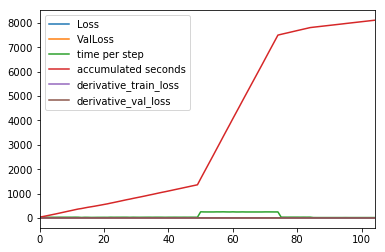
\includegraphics[width=0.9\linewidth, height=5cm]{./imgs/analysis_0_2_3.png} 
   \caption{Analysis 1 of run2.3}
   \label{fig:subAnalysisRun23}
   \end{subfigure}
   \begin{subfigure}{0.45\textwidth}
   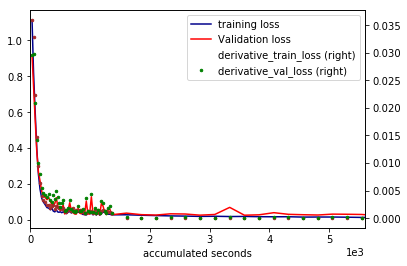
\includegraphics[width=0.9\linewidth, height=5cm]{./imgs/analysis_0_2_3plot.png}
   \caption{Analysis 2 of run2.3}
   \label{fig:subAnalysisRun23plot}
   \end{subfigure}
	
   \caption{Analysis for run 2.3}
   \label{fig:AnalysisRun23}
\end{figure}

\begin{figure}	
	\begin{subfigure}{0.45\textwidth}
	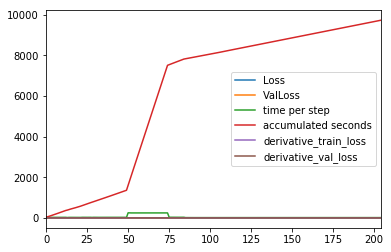
\includegraphics[width=0.9\linewidth, height=5cm]{./imgs/analysis_0_2_4.png} 
	\caption{Analysis 1 of run2.4}
	\label{fig:subAnalysisRun24}
	\end{subfigure}
	\begin{subfigure}{0.45\textwidth}
	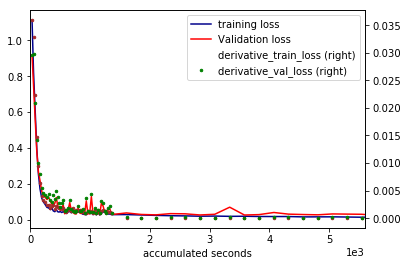
\includegraphics[width=0.9\linewidth, height=5cm]{./imgs/analysis_0_2_4plot.png}
	\caption{Analysis 2 of run2.4}
	\label{fig:subAnalysisRun24plot}
	\end{subfigure}
	 
	\caption{Analysis for run 2.4}
	\label{fig:AnalysisRun24}
 \end{figure}
 
\begin{figure}	
	\begin{subfigure}{0.45\textwidth}
	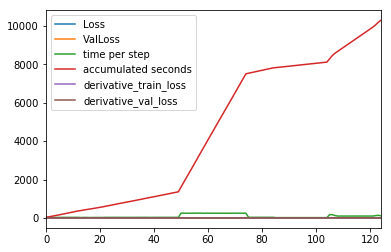
\includegraphics[width=0.9\linewidth, height=5cm]{./imgs/analysis_0_2_5.png} 
	\caption{Analysis 1 of run2.5}
	\label{fig:subAnalysisRun25}
	\end{subfigure}
	\begin{subfigure}{0.45\textwidth}
	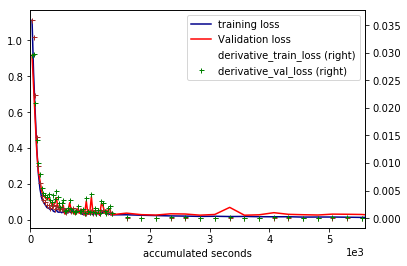
\includegraphics[width=0.9\linewidth, height=5cm]{./imgs/analysis_0_2_5plot.png}
	\caption{Analysis 2 of run2.5}
	\label{fig:subAnalysisRun25plot}
	\end{subfigure}
	 
	\caption{Analysis for run 2.5}
	\label{fig:AnalysisRun25}
 \end{figure}
 
\begin{figure}	
	\begin{subfigure}{0.45\textwidth}
	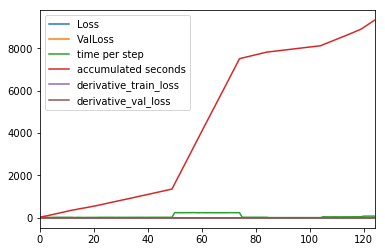
\includegraphics[width=0.9\linewidth, height=5cm]{./imgs/analysis_0_2_6.png} 
	\caption{Analysis 1 of run2.6}
	\label{fig:subAnalysisRun26}
	\end{subfigure}
	\begin{subfigure}{0.45\textwidth}
	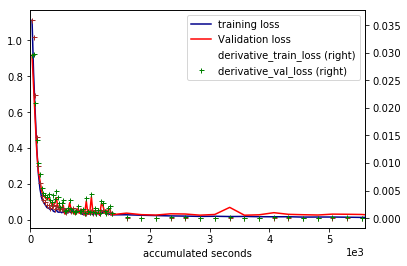
\includegraphics[width=0.9\linewidth, height=5cm]{./imgs/analysis_0_2_6plot.png}
	\caption{Analysis 2 of run2.6}
	\label{fig:subAnalysisRun26plot}
	\end{subfigure}
	 
	\caption{Analysis for run 2.6}
	\label{fig:AnalysisRun26}
 \end{figure}
 
\paragraph{Local minima}
The runs above seems to be stuck in the local minima, where only the scenes with heroin in proximity is in proirity, even though the performance for distant obejct recognition can be improved more. The loss and validation loss at minima converges to around 0.120 and 0.140. These values implies to train the model with a lower learning rate.

\subsection{Run 3}
Using lower learning rate, it will be slower to converge to a minima, but it will be lower than the one with higher learning rate.

\begin{table}
	\begin{center}
		\begin{tabular}{ l | c | c }
		\hline
		parameter & run3 & run3.1 \\ \hline
		learning rate & 0.0001 & 0.0001 \\ \hline
		batch size    & 16 & 8 \\ \hline
		num of epoch  & 50 & 25 \\ \hline
		accumulated trained epoch & 50 & 75 \\ \hline
		steps per epoch & 32 & 64 \\ \hline
		validation steps & 16 & 32 \\ \hline
		workers & 2 & 4  \\ \hline
		number of training sets & 4131 & 4131 \\ \hline
		input weights & new & 3 \\ \hline
		output weights & 3 & 3\_1\\ 		
		\hline \hline
		iou hero close &0.802 & 0.751 \\ \hline	  
		iou hero distant & 0.0402 & 0.018 \\ \hline
		final score & 0.259& 0.252 \\
		\hline
		\end{tabular}
		\caption{The parameters and validation results of Run 3}
		\label{tab:parameters3}
	\end{center}
\end{table}

Table~\ref{tab:parameters3} shows the new parameter sets to induct a lower global minima, instead of stuck in a local minima with higher learning rate. The only difference with run0 is the learning rate of one tenth of that in run 0. 
with this learning rate. The training was slower but achieved its own local minima to a half of the previous local minima. As can be seen in the file \href{run:./JupyterNotebooks/modeltrainingedit3.html}{modeltrainingedit3.html} and \href{run:./JupyterNotebooks/modeltrainingedit31.html}{modeltrainingedit31.html}, the output of FCN shows much traces random wavy stains, which indicates that the learning rate was too small to overcall the randomised weights after 50 times of epoch. After additional 25 epochs, these wavy stains in the output was removed, but still the overall performance was not as greate as the result of run 2.3.

\begin{figure}	
	\begin{subfigure}{0.45\textwidth}
	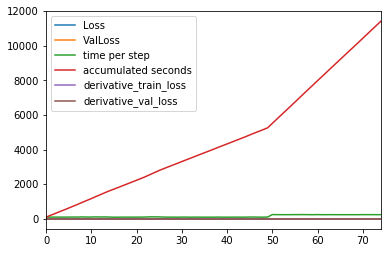
\includegraphics[width=0.9\linewidth, height=5cm]{./imgs/analysis_0_3.png} 
	\caption{Analysis 1 of run3}
	\label{fig:subAnalysisRun3}
	\end{subfigure}
	\begin{subfigure}{0.45\textwidth}
	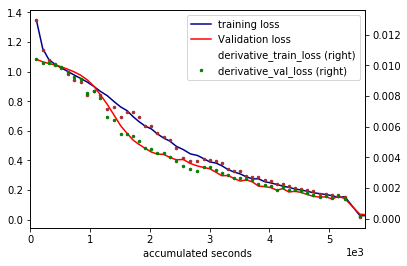
\includegraphics[width=0.9\linewidth, height=5cm]{./imgs/analysis_3plot.png}
	\caption{Analysis 2 of run3}
	\label{fig:subAnalysisRun3plot}
	\end{subfigure}
	 
	\caption{Analysis for run3}
	\label{fig:AnalysisRun3}
 \end{figure}

\subsection{Run 4}

A new learning rate which is half of run0 to run2 and five times bigger than run 3 was experimented and the hyperparameters are shown Table~\ref{tab:parameters4}. The majority of hyper parameters except learning rate was changed compared to run 3.
\begin{table}
	\begin{center}
		\begin{tabular}{ l | c | c | c }
		\hline
		parameter & run4 & run4.1 & run4.2 \\ \hline
		learning rate & 0.0005 & 0.0005 & 0.0005 \\ \hline
		batch size    & 16 & 16 & 8\\ \hline
		num of epoch  & 50 & 20 & 20\\ \hline
		accumulated trained epoch & 50 & 70 & 90\\ \hline
		steps per epoch & 32 & 32  & 32\\ \hline
		validation steps & 16 & 16 & 16\\ \hline
		workers & 2 & 4  & 4\\ \hline
		number of training sets & 4131 & 4131 & 4131\\ \hline
		input weights & new & 4 & 4\_1 \\ \hline
		output weights & 4 & 4\_1 & 4\_2\\ 		
		
		\hline \hline
		iou hero close & 0.623 & 0.875 & 0.808\\ \hline	  
		iou hero distant & 0.009 & 0.091 & 0.032\\ \hline
		final score & 0.202 & 0.318 & 0.275\\
		\hline
		\end{tabular}
		\caption{The parameters and validation results of Run 4}
		\label{tab:parameters4}
	\end{center}
\end{table}

In this run, the convergence to a local minima was faster than the run 3 and more stable than the run 0 to run 2. However the lower loss at 0.025 did not provide an accurate performance, instead it seems to be overfitted to the data. There is a sharp rise in loss at epoch 37 on the log graph for run 3. It does not mean that a weight set before epoch 37 may perform better and objective than the ones after epoch 37 - it could be less trained and the loss spike can be random near the local maxima. This implies the model was well overfitted to a part of the training set and it output a huge loss when it encountered the part of validation set which is totally different from the training set it was heavily overfitted. A dropout is needed to reduce such overfitting.

\begin{figure}	
	\begin{subfigure}{0.45\textwidth}
	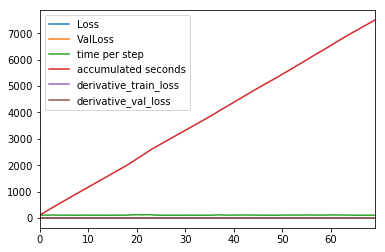
\includegraphics[width=0.9\linewidth, height=5cm]{./imgs/analysis_0_4.png} 
	\caption{Analysis 1 of run4}
	\label{fig:subAnalysisRun4}
	\end{subfigure}
	\begin{subfigure}{0.45\textwidth}
	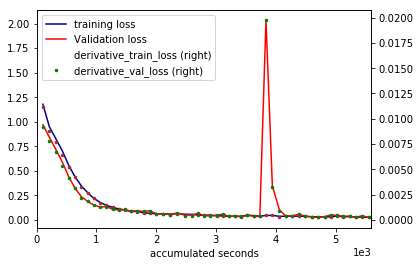
\includegraphics[width=0.9\linewidth, height=5cm]{./imgs/analysis_4plot.png}
	\caption{Analysis 2 of run4}
	\label{fig:subAnalysisRun4plot}
	\end{subfigure}
	 
	\caption{Analysis for run4}
	\label{fig:AnalysisRun4}
 \end{figure}
%------------------------------------------------

\subsection{Future Enhancements}

\paragraph{Different architecture}
One of my thought based on reviewing the scoring method of this project, the it might be more plausible to have two different streams of FCN to identify hero in distant and close ranges because mostly the model suffers inaccuracy in identification of distant objects. This is because of the single stream architecture FCN is more likely to specialised object recognition in proximity as the the first few layers of weights recognise the simple features of the heroin and the overall shape is recognised by the later layers. However, the shape of heroin does not have much details and size of is as small as the simple features can be detected by weights in the first layer of the network. To circumvent this, train another stream of FCN specialised for recognising heroin in distance by setting smaller filter sizes and feeding only training data sets with heroin in distance with other various objects and environment. By merging it carefully, actually this is the challenging part to do so and have incepeted the solution yet, the dual stream FCN may be able to recognise obejects both in proximity, and distance.
\paragraph{More data collection}
Due to the data deficiency in the provided data, especially the variety of scenes with a hero in distance, a well planned data acquisition is needed as shown in the data collection failure case of run 2.4 and run 2.5. 
\paragraph{Different Parameters}
At the end of writing this report, I realised that filter was 32 for all the experiments. I believe this could be one of the reasons why small objects, tiny image of hero in distance, could not be detected as good as the big objects. By increasing this filter size to 32, or even 64, small hero images might be detected better.
%----------------------------------------------------------------------------------------
\pagebreak
\section{Analysis}
%------------------------------------------------
\subsection{Advantage of the model}
With parameters supplied, this model can converge into a reasonable local minima within 1 hour to get the 43\% accuracy detection performance of he test data. This is a light and simple FCN also many rooms to improve too.

\subsection{Limitation of the model}
\paragraph{General purpose?}
Definately not enough training for many different objects, the training was limited to the object spawned in the simulated area. There is no animals, no cars. To make this recognised, more data sets are required. NVIDIA is conducting such general purpose data collection in \href{https://www.nvidia.com/en-us/deep-learning-ai/industries/ai-cities/}{smart cities} by using cameras installed in many locations in there. In addition, the size of neural network should become larger than this project to classify many more objects and this requires massive cloud system infrastructure to process the collected data.
Many people trying to make a general purpose classifer, however, only neural network itself might not be a model to do so becuase of its training time, model requirement, and the sensitivity of model to training data. There must be some more components to be added to create the novel generalised classifier.

%----------------------------------------------------------------------------------------
\newpage
\section{APPENDIX}

\subsection{Images}

\begin{figure}[ht]
	\begin{subfigure}{0.33\textwidth}
	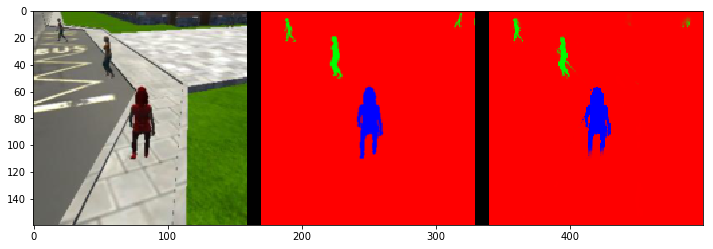
\includegraphics[width=0.9\linewidth, height=2cm]{./imgs/following_images23.png} 
	\caption{validataion - following images of run2.3}
	\label{fig:subfollowing_images23}
	\end{subfigure}
	\begin{subfigure}{0.33\textwidth}3
	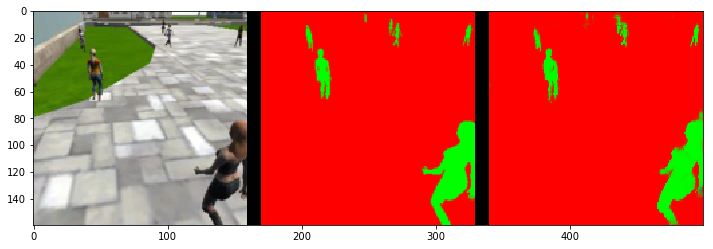
\includegraphics[width=0.9\linewidth, height=2cm]{./imgs/patrol_non_targ23.png}
	\caption{validataion - patrol without target of run2.3}
	\label{fig:subpatrol_non_targ23}
	\end{subfigure}
	\begin{subfigure}{0.33\textwidth}
	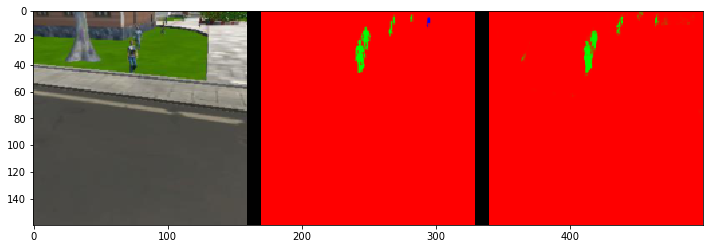
\includegraphics[width=0.9\linewidth, height=2cm]{./imgs/patrol_with_targ23.png}
	\caption{validataion - patrol with target of run2.3}
	\label{fig:subpatrol_with_targ23}
	\end{subfigure}

	\caption{validation images of run2.3}
	\label{fig:outputimages23}
\end{figure}

 \begin{figure}[ht]
	 \begin{subfigure}{0.33\textwidth}
	 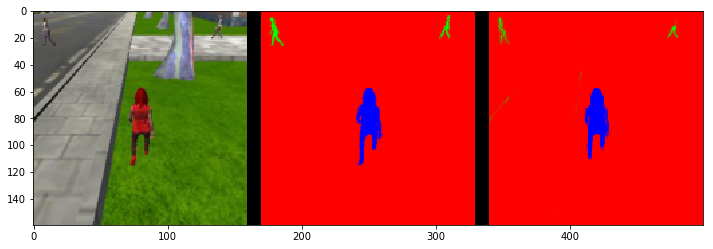
\includegraphics[width=0.9\linewidth, height=2cm]{./imgs/following_images24.png} 
	 \caption{validataion - following images of run2.4}
	 \label{fig:subfollowing_images24}
	 \end{subfigure}
	 \begin{subfigure}{0.33\textwidth}
	 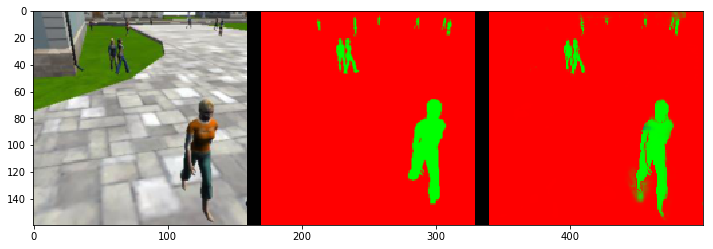
\includegraphics[width=0.9\linewidth, height=2cm]{./imgs/patrol_non_targ24.png}
	 \caption{validataion - patrol without target of run2.4}
	 \label{fig:subpatrol_non_targ24}
	 \end{subfigure}
	 \begin{subfigure}{0.33\textwidth}
	 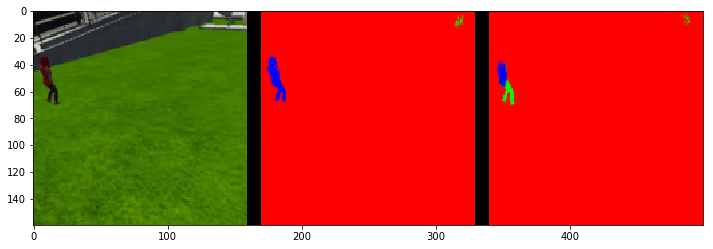
\includegraphics[width=0.9\linewidth, height=2cm]{./imgs/patrol_with_targ24.png}
	 \caption{validataion - patrol with target of run2.4}
	 \label{fig:subpatrol_with_targ24}
	 \end{subfigure}
 
	 \caption{validation images of run2.4}
	 \label{fig:outputimages24}
 \end{figure}


 \begin{figure}[ht]
	\begin{subfigure}{0.33\textwidth}
	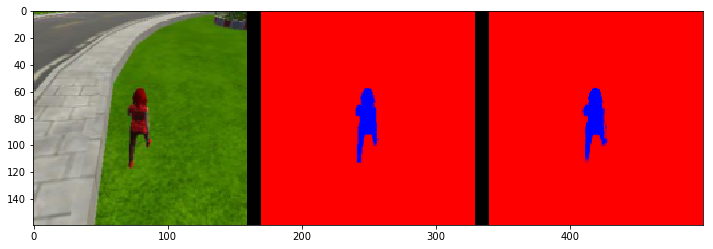
\includegraphics[width=0.9\linewidth, height=2cm]{./imgs/following_images25.png} 
	\caption{validataion - following images of run2.5}
	\label{fig:subfollowing_images25}
	\end{subfigure}
	\begin{subfigure}{0.33\textwidth}
	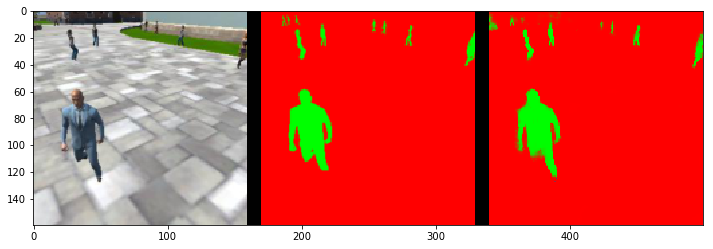
\includegraphics[width=0.9\linewidth, height=2cm]{./imgs/patrol_non_targ25.png}
	\caption{validataion - patrol without target of run2.5}
	\label{fig:subpatrol_non_targ25}
	\end{subfigure}
	\begin{subfigure}{0.33\textwidth}
	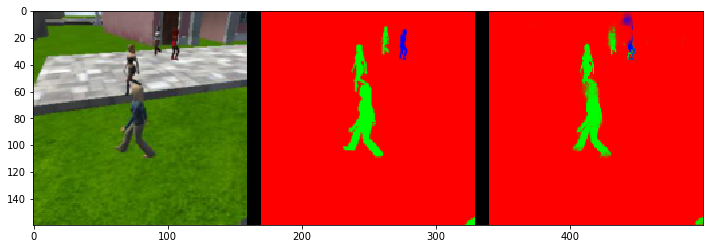
\includegraphics[width=0.9\linewidth, height=2cm]{./imgs/patrol_with_targ25.png}
	\caption{validataion - patrol with target of run2.5}
	\label{fig:subpatrol_with_targ25}
	\end{subfigure}

	\caption{validation images of run2.5}
	\label{fig:outputimages25}
\end{figure}

\begin{figure}[ht]
	\begin{subfigure}{0.33\textwidth}
	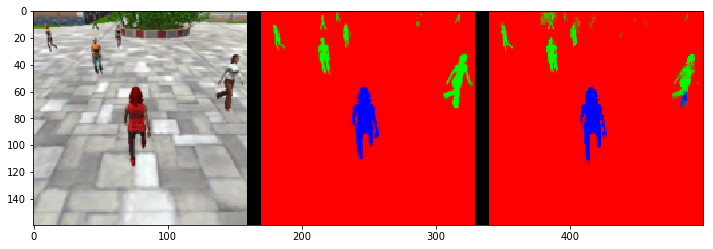
\includegraphics[width=0.9\linewidth, height=2cm]{./imgs/following_images26.png} 
	\caption{validataion - following images of run2.6}
	\label{fig:subfollowing_images26}
	\end{subfigure}
	\begin{subfigure}{0.33\textwidth}
	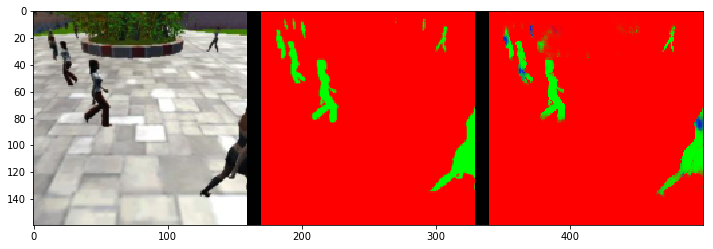
\includegraphics[width=0.9\linewidth, height=2cm]{./imgs/patrol_non_targ26.png}
	\caption{validataion - patrol without target of run2.6}
	\label{fig:subpatrol_non_targ26}
	\end{subfigure}
	\begin{subfigure}{0.33\textwidth}
	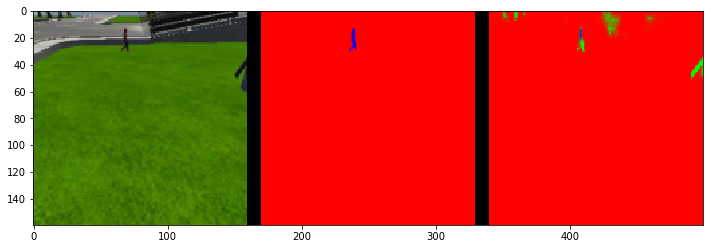
\includegraphics[width=0.9\linewidth, height=2cm]{./imgs/patrol_with_targ26.png}
	\caption{validataion - patrol with target of run2.6}
	\label{fig:subpatrol_with_targ26}
	\end{subfigure}

	\caption{validation images of run2.6}
	\label{fig:outputimages26}
\end{figure}

\begin{figure}[ht]
	\begin{subfigure}{0.33\textwidth}
	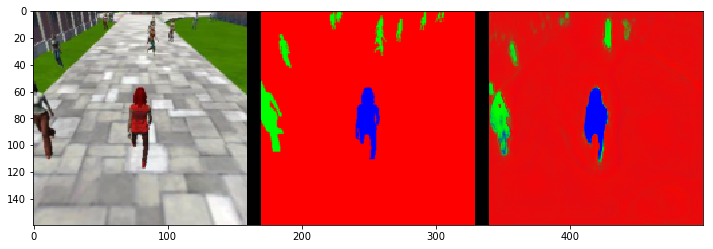
\includegraphics[width=0.9\linewidth, height=2cm]{./imgs/following_images3.png} 
	\caption{validataion - following images of run3}
	\label{fig:subfollowing_images3}
	\end{subfigure}
	\begin{subfigure}{0.33\textwidth}
	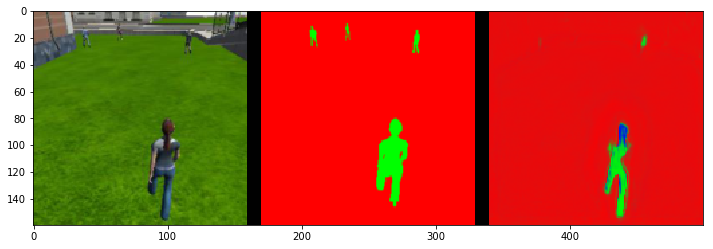
\includegraphics[width=0.9\linewidth, height=2cm]{./imgs/patrol_non_targ3.png}
	\caption{validataion - patrol without target of run3}
	\label{fig:subpatrol_non_targ3}
	\end{subfigure}
	\begin{subfigure}{0.33\textwidth}
	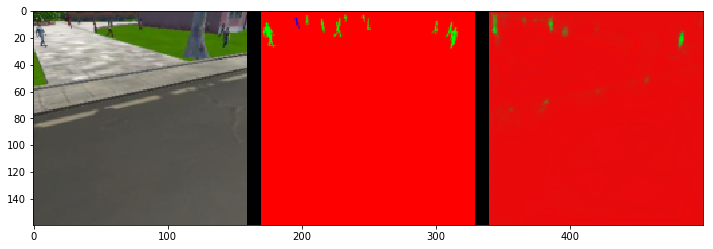
\includegraphics[width=0.9\linewidth, height=2cm]{./imgs/patrol_with_targ3.png}
	\caption{validataion - patrol with target of run3}
	\label{fig:subpatrol_with_targ3}
	\end{subfigure}

	\caption{validation images of run3}
	\label{fig:outputimages3}
\end{figure}

\begin{figure}[ht]
	\begin{subfigure}{0.33\textwidth}
	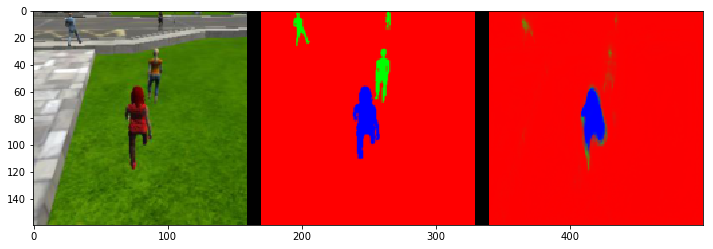
\includegraphics[width=0.9\linewidth, height=2cm]{./imgs/following_images3_1.png} 
	\caption{validataion - following images of run3}
	\label{fig:subfollowing_images31}
	\end{subfigure}
	\begin{subfigure}{0.33\textwidth}
	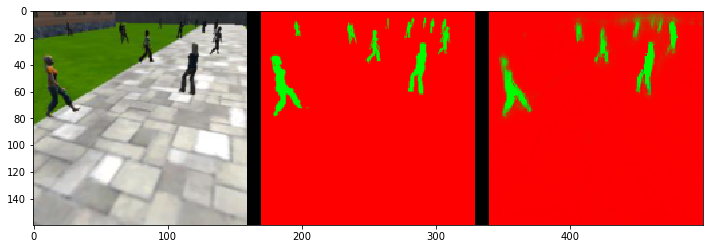
\includegraphics[width=0.9\linewidth, height=2cm]{./imgs/patrol_non_targ3_1.png}
	\caption{validataion - patrol without target of run3}
	\label{fig:subpatrol_non_targ31}
	\end{subfigure}
	\begin{subfigure}{0.33\textwidth}
	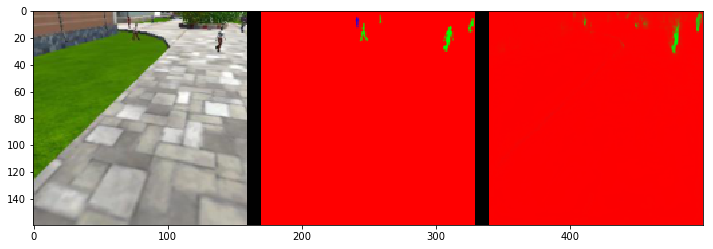
\includegraphics[width=0.9\linewidth, height=2cm]{./imgs/patrol_with_targ3_1.png}
	\caption{validataion - patrol with target of run3}
	\label{fig:subpatrol_with_targ31}
	\end{subfigure}

	\caption{validation images of run3}
	\label{fig:outputimages31}
\end{figure}

\begin{figure}[ht]
	\begin{subfigure}{0.33\textwidth}
	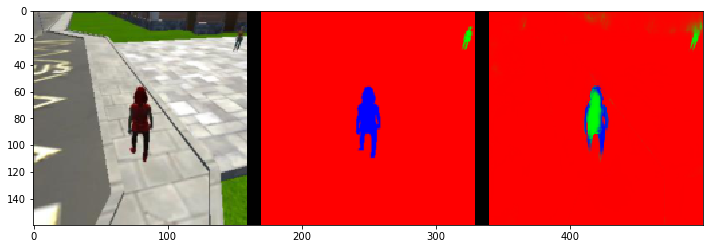
\includegraphics[width=0.9\linewidth, height=2cm]{./imgs/following_images4.png} 
	\caption{validataion - following images of run4}
	\label{fig:subfollowing_images4}
	\end{subfigure}
	\begin{subfigure}{0.33\textwidth}
	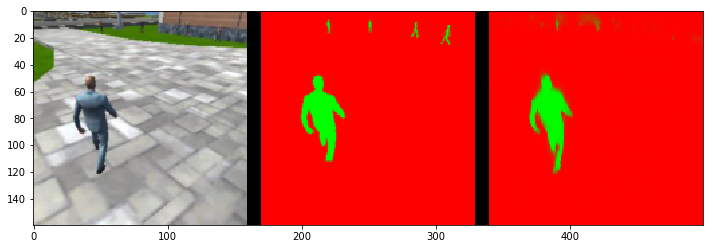
\includegraphics[width=0.9\linewidth, height=2cm]{./imgs/patrol_non_targ4.png}
	\caption{validataion - patrol without target of run4}
	\label{fig:subpatrol_non_targ4}
	\end{subfigure}
	\begin{subfigure}{0.33\textwidth}
	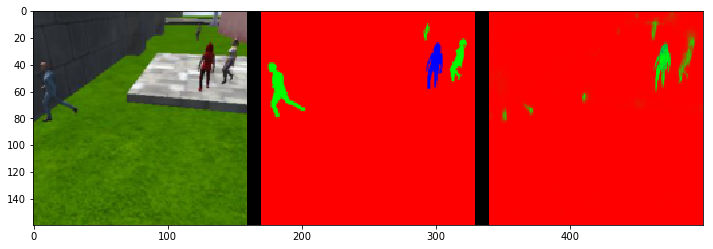
\includegraphics[width=0.9\linewidth, height=2cm]{./imgs/patrol_with_targ4.png}
	\caption{validataion - patrol with target of run4}
	\label{fig:subpatrol_with_targ4}
	\end{subfigure}

	\caption{validation images of run4}
	\label{fig:outputimages4}
\end{figure}

\begin{figure}[ht]
	\begin{subfigure}{0.33\textwidth}
	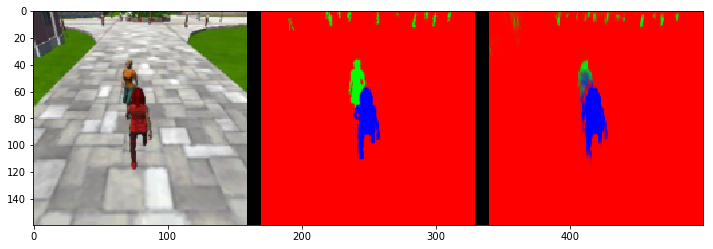
\includegraphics[width=0.9\linewidth, height=2cm]{./imgs/following_images4_1.png} 
	\caption{validataion - following images of run41}
	\label{fig:subfollowing_images41}
	\end{subfigure}
	\begin{subfigure}{0.33\textwidth}
	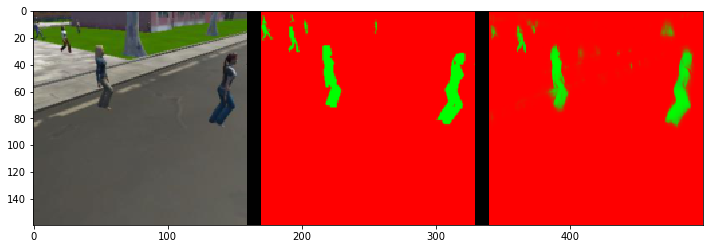
\includegraphics[width=0.9\linewidth, height=2cm]{./imgs/patrol_non_targ4_1.png}
	\caption{validataion - patrol without target of run41}
	\label{fig:subpatrol_non_targ41}
	\end{subfigure}
	\begin{subfigure}{0.33\textwidth}
	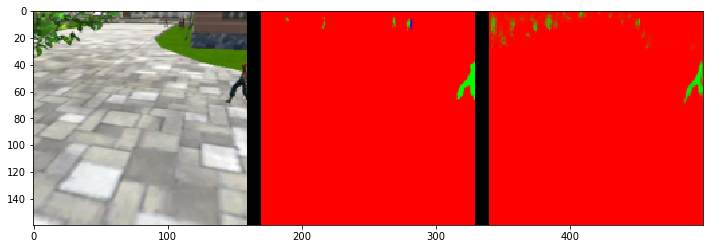
\includegraphics[width=0.9\linewidth, height=2cm]{./imgs/patrol_with_targ4_1.png}
	\caption{validataion - patrol with target of run41}
	\label{fig:subpatrol_with_targ41}
	\end{subfigure}

	\caption{validation images of run41}
	\label{fig:outputimages41}
\end{figure}

\end{document}
